\documentclass{CCI2020}

\pagestyle{empty}
\fancypagestyle{firstpage}{
\fancyhf{}
\lhead{\includegraphics[width=20mm]{images/IFSS-logo}}
\chead{
\vspace{5mm}
\textbf{
به‌نام خدا}}
\rhead{
\includegraphics[width=20mm]{images/logo.jpg}}
\cfoot{
\textbf{
}}
}
\renewcommand{\headrulewidth}{0.0pt}

\title{
تصمیم‌گیری مالی و محاسبه جریان نقدی آزاد
}
\date{}
\author[1]{محمّدمهدی خانی}
\author[2]{پارسا فدائی خدمت}
\author[3]{علیرضا زمانی}
\affil[1]{
دانشجوی مهندسی کامپیوتر ورودی 97 دانشگاه شهید بهشتی، mm.y.khani@gmail.com
}
\affil[2]{
 دانشجوی مهندسی کامپیوتر ورودی 97 دانشگاه شهید بهشتی، parsafadaei@yahoo.com
}
\affil[3]{
 دانشجوی مهندسی کامپیوتر ورودی 97 دانشگاه شهید بهشتی، alireza-zamani@outlook.com
}


\begin{document}
\maketitle
\thispagestyle{firstpage}
\begin{abstract}
در این مقاله در مورد نحوه اتخاذ یک تصمیم مالی در راستای قبول یا رد کردن یک پروژه بحث می‌شود. مهم ترین ویژگی یک پروژه قابل قبول، ارزش‌آفرینی این پروژه در طول زمان است. برای اندازه‌گیری سودمندی یک پروژه در طول زمان شاخص‌های زیادی تعریف شده که یکی از پرکاربردترین آنها شاخص ارزش خالص فعلی است.
برای محاسبه ارزش خالص فعلی نیازمند محاسبه جریان نقدی آزاد هستیم که به صورت مفصل به نحوه محاسبه آن می‌پردازیم.
در آخر در مورد کاربرد شاخص ‌های تصمیم‌گیری مالی در عمل می‌پردازیم و نشان میدهیم که تا حد خوبی این شاخص‌ها قابل اعتماد هستند.

 \end{abstract}
\begin{keywords}
جریان مالی، ارزش خالص فعلی، جریان نقدی آزاد،تنزیل جریان نقدی، سپر مالیاتی 
\end{keywords}


\section{مقدمه}
ارزش پول در زمان متغییر است و بجز بعضی کشور های محدود، ارزش پول در زمان افت می‌کند و شاید پول فردا همان پول امروز نباشد. مردم کشورهایی مثل ونزوئلا این اصل را بخوبی حس می‌کنند. در ونزوئلا دولت هر چند ماه یکبار حقوق کارکنانش را چند برابر میکند و همین نکته بیانگر این است که ارزش پول در ونزوئلا بسرعت و بشدت در حال افول است.



\begin{figure}[htb]\centering
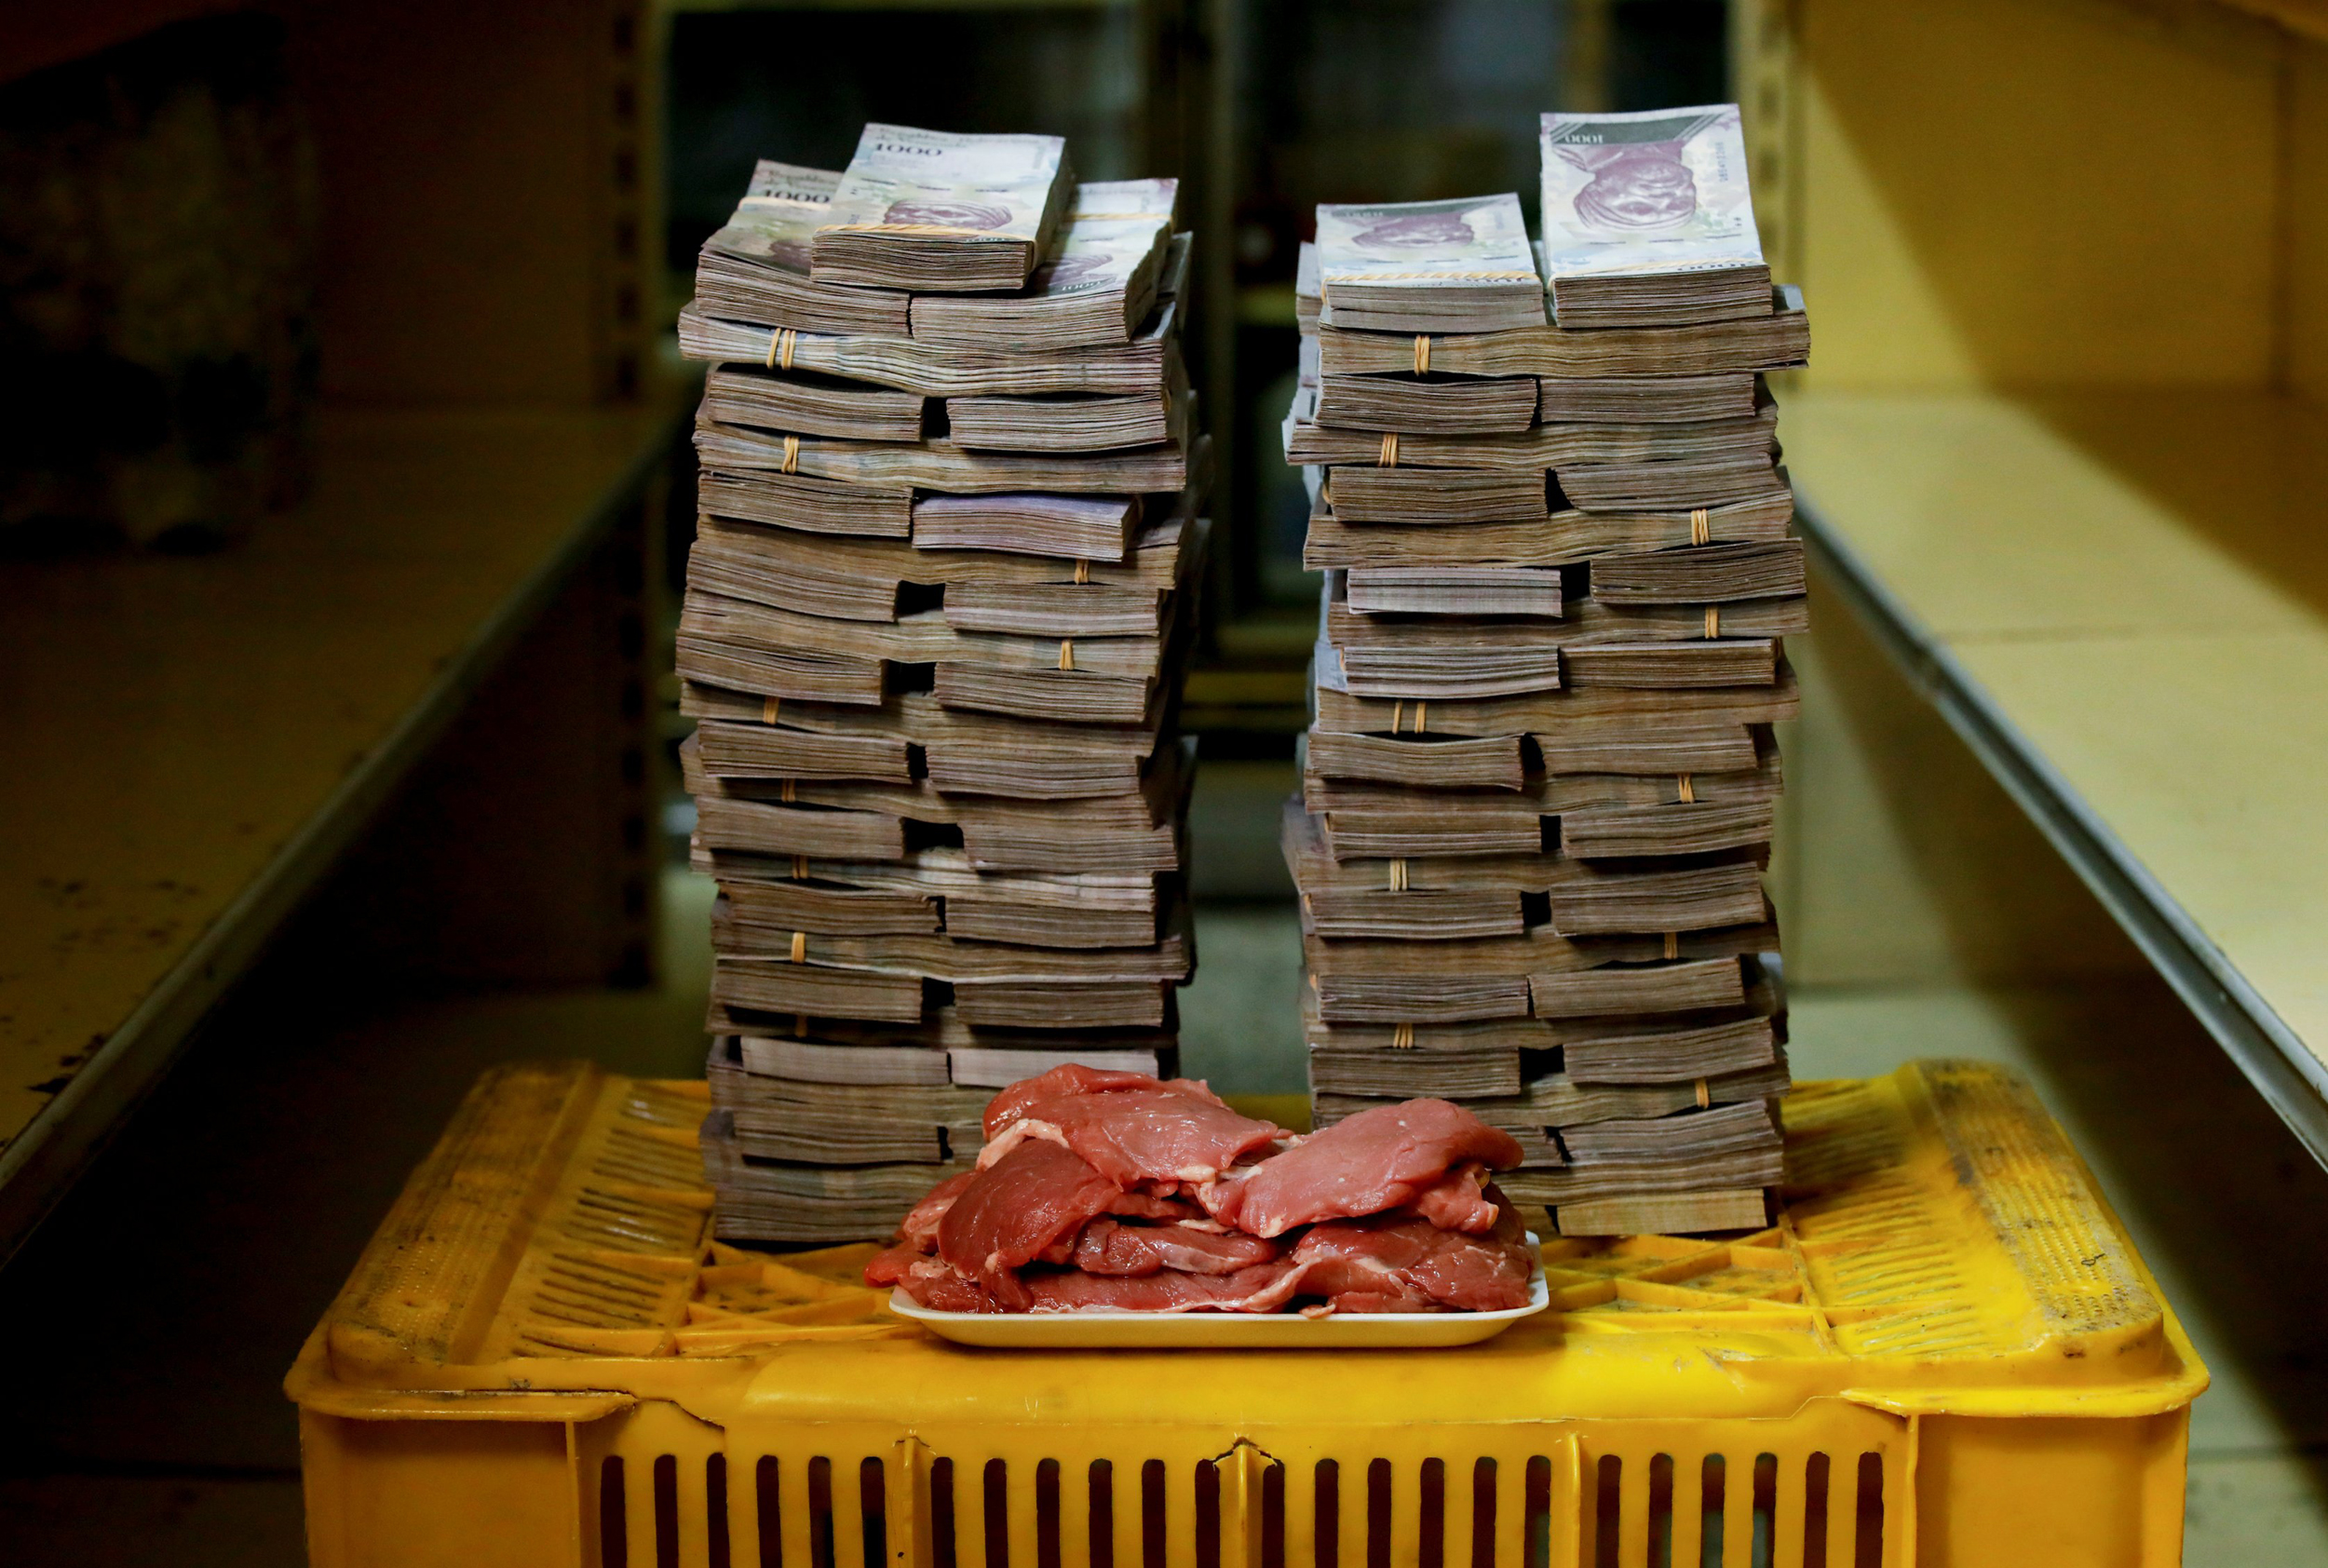
\includegraphics[height=0.5\hsize]{images/venezuelaMoney.jpg}
\caption{برای خرید 1 کیلوگرم گوشت در ونزوئلا باید مبلغ 
9,500,000
بولیوار بپردازید.
\cite{venezuela}}
\end{figure}

نرخ تورم در این کشور حدود 3000 درصد است.
تورم در لغت به معنی ورم کردن، دمیده شدن و بزرگ شدن در عین خالی بودن است.
در علم اقتصاد نیز پدیده تورم به خاطر افزایش قیمت بدون پشتوانه به‌وجود می‌آید. به این معنی که سطح عمومی قیمت کالاها و خدمات به شکلی نامنظم و غیرمتناسب با قدرت خرید و ارزش پول، در یک بازه زمانی مشخص افزایش یابد. تورم ارتباط تنگاتنگی با کاهش ارزش پول دارد و در کشوهایی که تورم بالایی دارند مفهموم ارزش پول در زمان، حتی توسط افرادی که تحصیلات آکادمیک ندارند خیلی خوب درک می‌شود.

شاخص‌های زیادی برای تعیین میزان سودمندی یک تصمیم مالی وجود دارد که یکی از کاربردی‌ترین آنها که بیشتر شرکت‌ها نیز از همین شاخص استفاده می‌کنند، شاخص NPV\LTRfootnote{Net present value}
 است. هر چه میزان
 NPV
 مثبت‌تر باشد نشان‌دهنده این است که پروژه مورد نظر سودمندتر است و اگر NPV منفی باشد نشان ‌دهنده این است که پروژه، پروژه سودآوری نیست و نباید آن پروژه را قبول کرد. 

\section{قانون ارزش خالص فعلی}

برای تصمیم‌گیری در لحظه و برای اینکه یک پروژه با توجه به آورده‌ها و هزینه‌هایی که در طول زمان دارد نمی‌توانیم به یک جمع و تفریق کردن ساده درآمدها و هزینه‌ها اکتفا کنیم.
NPV
یا همان ارزش خاص فعلی،
تفاوت میان ارزش کنونی جریانات نقدی ورودی و ارزش کنونی جریان نقدی خروجی است.
NPV
برای بودجه‌بندی سرمایه مورد استفاده قرار می‌گیرد تا احتمال سرمایه‌گذاری محاسبه‌شده یا پروژه را تحلیل کند.
فرمول ساده شده قانون 
NPV
به صورت زیر است.
\begin{equation}
NPV =  {\text{\rl{ارزش فعلی درآمد}}} - {\text{\rl{ارزش فعلی هزینه}}}
\end{equation}
این توصیف از 
NPV
یک مفهموم عام را از این شاخص به ذهن متبادر می‌کند. این شاخص در واقع به ما کمک می‌کند که ارزش فعلی و سود قبول پروژه در لحظه حال را محاسبه کنیم و اگر این سود منفی بود به معنای زیان‌ده بودن پروژه است.


\subsection{محاسبه ارزش خالص فعلی}
برای محسابه 
NPV
در عمل از فرمول 2 که فرمول دقیق‌تر و کامل‌تری است استفاده می‌شود.
\begin{equation}
NPV = FCF\LTRfootnote{Free cash flow} +  \frac{FCF_{0}}{(1+R)}+  \frac{FCF_{1}}{(1+R)^{2}} + ...
\end{equation}
در واقع 
NPV
با استفاده از تنزیل ارزش جریان‌های نقدی آزاد به زمان حال 
DCF)\LTRfootnote{Discounted cash flow})
محاسبه می‌شود. در این بیان از 
NPV
ارزش جریان های نقدی آزاد در زمان های مختلف متاسب با زمان (بصورت نمایی) و متناسب با مقدار نرخ بهره (بصورت خطی) کاهش می‌یابند. 

در این رابطه 
توان اعدادی که در مخرج آمده‌اند
زمان انجام هزینه یا بدست آمدن درآمد هستند 
R
نرخ بهره(حاصل‌ضرب نرخ سود، نرخ ریسک و نرخ تورم قابل پیش‌بینی) 
و مقدار 
FCF
بیانگر مقدار کمی درآمد یا هزینه بر اساس جریان نقدینگی است که در ادامه به صورت مفصل به این مفهوم خواهیم پرداخت.
 
\subsection{چه شرکت‌هایی از NPV استفاده می‌کنند؟}
در بین شرکت‌های مالی بزرگ شاخص 
NPV
بالاترین رتبه کاربرد را دارد و در شرکت‌های مالی شخصی کوچک، این شاخص  در جایگاه دوم قرار دارد. که همین نکته تائیید‌کننده کابردی بودن شاخص 
NPV
است.
برخلاف تصور افراد غیر‌متخصص، ارزش خالص فعلی روشی معتبر برای تصمیم‌گیری‌های مالی است.

\section{جریان نقدی آزاد}
جریان نقدی آزاد، جریان نقدی حاصل از عملیات بعد از کسر مالیات، بدون احتساب بدهی‌ها و هزینه‌های بهره شرکت است؛ بنابراین، جریان نقدی آزاد، وجوه نقدی است، که بعد از پوشش دادن نیازهای سرمایه‌گذاری و سرمایه در گردش و با فرض نبود بدهی، در دسترس شرکت قرار می‌گیرد. در شرکت‌های بدون بدهی یا فاقد اهرم مالی، جریان نقدی آزاد، همان جریان نقدی حقوق صاحبان سهام است.

جریان نقدی آزاد عبارت است از سود عملیاتی پس از مالیات، به اضافه هزینه‌های غیرنقدی پس از کسر سرمایه‌گذاری (افزایش در تغییرات) در سرمایه در گردش، اموال، ماشین‌آلات، تجهیزات و سایر دارایی‌ها. جریان‌های نقدی آزاد اغلب این امکان را فراهم می‌کند، تا مدیریت در صورت نبود ساختار حاکمیت شرکتی مناسب، به دستکاری سود اقدام کند. شرکت‌هایی که دارای جریان‌های نقدی آزاد بیشتری هستند، با مشکلات هزینه نمایندگی بیشتری روبرو می‌باشند؛ به‌ویژه در شرکت‌هایی که فرصت‌های سرمایه‌گذاری کم بوده یا از رشد کم برخوردارند.

به عبارت دیگر 
جریان نقدی آزاد یا  جریان نقد در اختیار شرکت پس از خروج وجه نقد و برای پوشش عملیات جاری و حفظ دارایی‌های شرکت است. جریان نقدی آزاد هزینه‌های غیر نقدی مانند استهلاک دارایی‌ها و تجهیزات را از صورت سود و زیان حذف می‌کند. جریان نقدی آزاد این فرصت را به مدیران یک شرکت می‌دهد که به دنبال فرصت‌های افزایش بازدهی باشند و برنامه‌های توسعه محصول، گسترش کسب‌وکار، پرداخت سودهای نقدی و کاهش بدهی‌ها را به سرانجام برسانند.\cite{corporatefinanceinstitute.com}


جریان نقدی آزاد از دو بخش جریان نقدی ورودی و جریان نقدی خروجی تشکیل شده است.
این جریان همه وجوه نقدی است که به شرکت وارد می‌شود. این وجه نقد از طریق فروش محصول تولیدی، فروش دارایی و سود سرمایه‌گذاری حاصل می‌شود

این جریان نیز وجوه نقدی است که از شرکت خارج می‌شود؛ مانند وجه نقد لازم برای خرید مواد اولیه و تجهیزات، حقوق کارکنان، هزینه‌های عملیاتی و بهره وام.

براساس توضیحات داده شده، جریان نقدی آزاد براساس فرمول زیر قابل محاسبه است:
\begin{equation}
FCF =  {\text{\rl{جریان نقدی ورودی}}} - {\text{\rl{جریان نقدی خروجی}}
\end{equation}در ادامه برای محاسبه دقیق جریان نقدی آزاد رابطه 4 را معرفی می‌کنیم و در مورد اجزای آن بحث می‌کنیم.


\subsection{محاسبه جریان نقدی آزاد}

برای محاسبه جریان نقدی آزاد میتوان از رابطه 4 استفاده کرد. شاید بخش‌هایی از این رابطه دقیقا قایل اندازه‌گیری نباشند و هرچه ابعاد مسئله بزرگ‌تر شود این احتمال بیشتر است. اما تاحد ممکن باید در تخمین اجزای مختلف این فرمول دقت‌عمل بخرج داد تا نتیجه پایانی یک نتیجه قابل اتکا و مطمئن باشد.\cite{coursera.org/learn/wharton-finance.com}

ممکن است در نگاه اول، مهارت تخمین‌زدن و برآورد‌کردن، مهارت کوچک و ساده‌ای به نظر برسد.واقعیت این است که مهارت تخمین‌زدن می‌تواند نقش مهمی در موفقیت یا شکست شرکت داشته باشد و در صورتی که نتایج غلطی از تخمین‌های غلط حاصل شود، به مراتب زیان‌بار‌تر از نداشتن یک دید کلی نسبت به مسئله است.
\begin{equation}
FCF =  {(\text{\rl{درآمد}}} - {\text{\rl{هزینه}} - {\text{\rl{استهلاک}} )} *  {(\text{\rl{1}}} - {\text{\rl{مالیات}})}+\text{\rl{استهلاک}} -

\text{\rl{هزینه‌های سرمایه گذاری}}}-
\text{\rl{تغییرات دارایی‌های جاری}}}
\end{equation}



\subsubsection{درآمد}
درآمد با سود متفاوت است. فرمول درآمد یک شرکت تولیدی از رابطه زیر محاسبه میشود:
\begin{equation}
\text{\lr{درآمد}}  =  {(\text{\rl{قیمت}}} * {\text{\rl{اندازه بازار}} * {\text{\rl{سهم ما از بازار}} )}
\end{equation}

اندازه بازار یعنی تمام متقاضیان محصول تولیدی یک شرکت که این متقاضیان، مشتریان بالقوه این شرکت تولیدی محسوب می‌شوند ولی همه این مشتریان الزاما از این شرکت بخصوص خرید نمی‌کنند. 

آن درصد از مشتریانی که از این شکرت بخصوص خرید می‌کنند را سهم این شرکت از کل بازار می‌نامند که در واقع مشتریان بالفعل هستند که واقعا از ما خرید می‌کنند.
منظور از قیمت هم قیمت نهایی یک واحد از کالای تولیدی است که توسط خود شرکت بفروش می‌رسد. این کالا می‌تواند مستقیما به مصرف‌کننده نهایی فروخته شود یا با قیمتی متفاوت به شرکت‌های پخش فروخته شود و در واقع توضیع این محصولات به شرکت های پخش واگذار شود. این تفاوت قیمت نیز باید در رابطه بالا لحاظ شود.
\subsubsection{استهلاک}
استهلاک ازجمله اصطلاحاتی است که در زندگی روزمره ما بطور معمول استفاده می‌شود و مستهلک شدن وسایل بمرور زمان و در اثر استفاده امری طبیعی است. هر وسیله و ابزاری که برحسب نیاز خریداری کنیم، در اثر استفاده از آن مستهلک شده و کارایی خود را به تدریج از دست می‌دهد. درنتیجه استهلاک ازجمله مواردی است که هزینه تعمیرات وسایل و تجهیزات و حتی گاهی خرید ابزار جدید را به ما تحمیل می‌کند.

دارایی‌های ثابت یک شرکت نیز با گذشت زمان و با استفاده مکرر دچار فرسودگی، فرسایش و کهنگی ناشی از استفاده خواهند شد و به تدریج فایده خود را از لحاظ انجام دادن کار ها از دست می‌دهند.
حسابداری سعی می‌کند این کاهش فایده رسانی این دارایی‌های ثابت را به روش معقول و منطقی محاسبه کند که به آن هزینه استهلاک می‌گویند.

در این فرمول استهلاک یک‌بار از درآمد کم شده و یک‌بار دیگر پس از کسر مالیات از سود، به
\rl{FCF}
باز می‌گردد. که دلیل آن مسئله سپر مالیاتی است. در این تکنیک ابتدا هزینه استهلاک از درآمد کم می‌شود تا مقدار سرمایه‌ای که مالیات به آن تعلق می‌گیرد کم شود، و پس از کسر مالیات مجددا به درآمد اضافه می‌گردد. دلیل این بازگشت مجدد این است که استهلاک بصورت فیزیکی مبلغی از 
\rl{FCF}
کم نمی‌کند.
\cite{accountingtools.com/articles/2017/5/6/depreciation-expense}

\subsubsection{سپر مالیاتی چیست؟}
سپر مالیاتی یک استراتژی قانونی است که "اجتناب از مالیات" نامیده می شود. در مقابل آن "فرار مالیاتی"  قرار دارد که کسر غیرقانونی عمدی، پنهان کردن یا گزارش نکردن درآمد است که پرداخت نکردن آن با مجازات‌ها و تعقیب کیفری احتمالی را به همراه دارد.
 

در این تکنیک به این صورت عمل می‌شود که به عنوان یک شخص یا کسب وکار می‌توانید خریدها و فعالیت‌هایی انجام دهید که موجب کسر مالیات شود.
شما می‌توانید این کار را به طور تصادفی انجام دهید، در هر زمان که بخواهید هرچه می‌خواهید خریداری کنید. یا می‌توانید عمداً با برنامه‌ریزی خرید برای استفاده از سپرهای مالیاتی‌، در مالیات پس انداز کنید.
به عنوان نمونه‌هایی از سپر مالیاتی در زمینه‌های مختلف می‌توان به موارد زیر اشاره کرد. 
 مثلا کمک‌های خیرخواهانه در شرایطی هم برای افراد و هم برای مشاغل  موجب کسر مالیات می‌شود. شرکت ها می‌توانند کمک‌های خیرخواهانه را با وجود برخی محدودیت‌ها انجام دهند.
وام مسکن یک سپر مالیاتی کلاسیک برای افراد و مشاغل است.   نکته مهم این است که مبلغ پرداخت وام مسکن قابل کسر نیست؛ این مورد شامل هزینه سود حاصل از وام  است.
مشاغل می‌توانند برای خرید ملک، تجهیزات، مبلمان و وسایل نقلیه و وسایل نقلیه (اما نه زمین) هزینه استهلاک بپردازند. استهلاک اساساً روشی برای توزیع هزینه خرید دارایی تجاری در طول عمر آن دارایی است.
استهلاک تسریع شده به شما امکان می دهد مقدار بیشتری از دارایی را در یکی دو سال اول استهلاک کنید و این یک نمونه عالی از سپر مالیاتی است.

\begin{figure}[htb]\centering
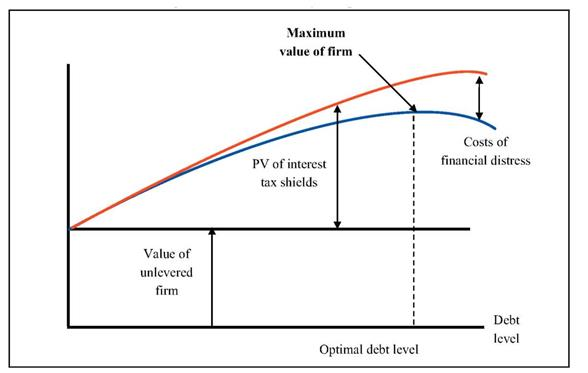
\includegraphics[height=0.6\hsize]{images/TaxShield.jpg}
\caption{تاثیرات استفاده از تکنیک سپر مالیاتی
\cite{TaxShield}}
\end{figure}

\subsubsection{مالیات}
مالیات، یک نوع هزینه اجتماعی است که همه افراد یک جامعه در راستای بهره‌برداری از امکانات و منابع کشورشان موظفند آن را پرداخت کنند تا توانایی جایگزینی این امکانات و منابع فراهم شود.مالیات در واقع انتقال بخشی از درآمد‌های جامعه به دولت یا بخشی از سود فعالیت‌های اقتصادی است که نصیب دولت می‌شود، زیرا ابزار و امکانات دست یابی به درآمد و سود‌ها را دولت فراهم ساخته ‌است.

مالیات در کشورهای مختلف و بسته به حجم کسب و کار و نوع کسب و کار متفاوت است. مثلا در ایران شرکت‌های دانش بنیان سطح یک تا 2 سال معاف از پرداخت مالیات هستند. و نرخ مالیات بسته به زمان و مکان و موقعیت کسب و کار متفاوت است و مدام در حال تغییر.
در سال 2019 از بین 10 کشوری که بیشترین مالیات بر درآمد را داشتند، 7 کشور اروپایی حضور داشت. به طور متوسط مالیات در کشور های پیشرفته بیشتر از مالیات کشور‌های جهان سوم است.


\begin{figure}[htb]\centering
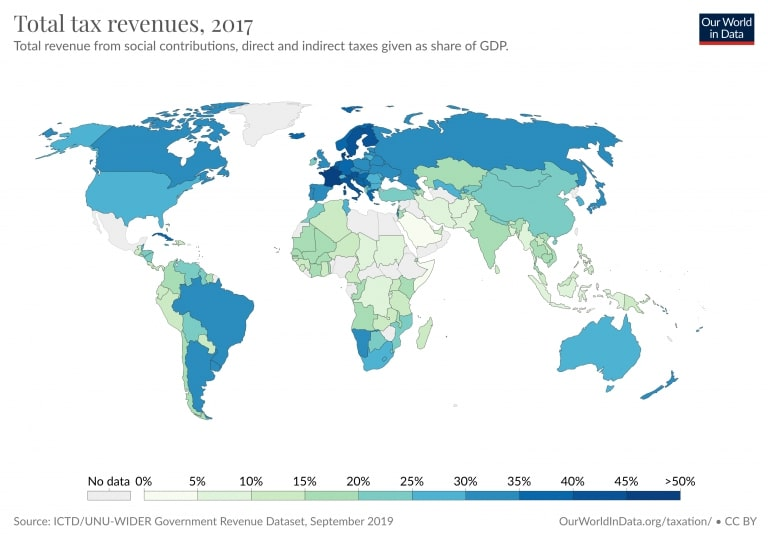
\includegraphics[height=0.7\hsize]{images/worldTax.jpg}
\caption{پراکندگی کشورهای با بیشترین نرخ مالیات
\cite{worldTax}}
\end{figure}

\subsubsection{هزینه‌های سرمایه‌گذاری}
سرمایه‌گذاری‌های ثابت منابع مادی مورد نیاز برای ساخت و تجهیز پروژه هستند.
هزینه سرمایه، به هرگونه هزینه‌ ای گفته می‌شود که به سرمایه تبدیل شده است و معیاری موثر در جریان مالی محسوب می‌شود. در واقع این گروه از این هزینه‌ها یک نوع هزینه صرف نیستند و در واقع یک نوع سرمایه گذاری هستند. مثلا شرکتی که یک سوله صنعتی با دستگاه‌های صنعتی را تجهیز می‌کند نوعی از سرمایه‌گذاری را انجام داده است.

هزینه هایی مثل خریدن زمین، ساخت و ساز سوله، خرید تجهیزات و ... نمونه‌هایی از هزینه‌های سرمایه‌گذاری هستند.

\subsubsection{تغییرات دارایی‌های جاری}
ابتدا باید بدانیم دارایی‌های جاری چیست. دارایی‌های جاری یا همان
NWC\LTRfootnote{Net working capital}
عبارت‌اند از مجموع حساب‌های دریافتنی بعلاوه موجودی انبار و پول، منهای حساب‌های پرداختنی.
حساب پرداختنی زمانی به وجود می‌آید که شرکت اجناس یا خدماتی را به صورت نسیه از تامین‌کنندگان خود خریداری می‌کند. حساب‌پرداختنی باید طی یک سال مالی یا در یک چرخه‌ی عملیاتی (که طولانی‌تر است) پرداخت شود. حساب پرداختنی یکی از رایج‌ترین شکل‌های بدهی‌های جاری در ترازنامه است. در حسابداری دو طرفه در صورتی که اصطلاح حساب‌پرداختنی برای یک نهاد یا شرکت به کار گرفته شود ، برای نهاد مقابل حساب دریافتنی محسوب می‌شود.

حساب‌های دریافتنی فروش اعتباری یک کسب‌وکار را نشان می‌دهند که هنوز توسط مشتریان به طور کامل پرداخت نشده‌اند. شرکت‌ها به مشتریان خود اجازه می‌دهند که در یک بازه زمانی معقول و گسترده و با شرایط مورد توافق، پول خرج کنند. مشتری می‌تواند برای معاملاتی مشخص و پرداخت زودهنگامِ بدهی خود به شرکت، تخفیف دریافت کند.

\section{کابرد شاخص‌های تصمیم‌گیری در عمل}
همان‌طور که پیش‌تر نیز اشاره شد، شاید در نگاه اول برای افرادی که اطلاعی از حساب‌داری ندارند و برای مراودات مالی شخصی خودشان هم از هیچ یک از اصول و قواعد حساب‌داری استفاده نمیکنند، شاخص های تصمیم‌گیری از جمله ارزش خالص فعلی یک شاخص زینتی و در عمل غیر قابل استفاده تلقی شود. احتمالات نانوشته و خطاهای محاسبه نشده تا حدودی در دقت این شاخصه‌ها تاثیر گذارند و هر چقدر که ابعاد مسئله‌ای که آن را با  شاخص‌های ارزیابی اندازه می‌گیرم بیشتر باشد احتمال خطا بیشتر است. برای مثال، اندازه گیری طول یک میز شاید خطایی در حدود چند سانتی‌متر داشته باشد ولی اندازه گیری طول یک اتوبان احتمالا خطایی به اندازه چند ده متر خواهد داشت. همین مساله در تصمیم‌گیری‌های مالی نیز برقرار است. برنامه پروژه چند ساله یک شرکت بزرگ خطا‌ها و گزینه‌های در نظرگرفته نشده بیشتری دارد تا برنامه 6 ماهه یک شرکت استارت‌آپی.
فرض کنید الان سال 2018 است و شرکت شما مسئولیت اجرا و پیاده‌سازی پروژه ساختن یک شهربازی بزرگ در تهران را بعهده گرفته و در قرارداد مرقوم شده که تا 5 سال، 10 درصد از سود سالانه شهربازی به شرکت شما پرداخت شود و همه شاخص‌های تصمیم‌گیری مالی هم این‌طور نشان می‌دهند که این تصمیم‌گیری یک تصمیم‌گیری پول‌ساز و سودآفرین است. اما شما بعد از حدود 2 سال با پدیده‌ای به نام ویروس کرونا مواجه می‌شوید که به یکباره کل این محاسبات را بر هم می‌زند و حتی ممکن است باعث شود این پروژه به شما ضرر برساند. آیا این مورد دلیلی بر ناکارآمدی شاخص‌های تصمیم‌گیری است؟ مشخصا نه! اگر از این شاخص‌های تصمیم‌گیری استفاده نمی‌کردید در شرایط عادی هم نمی‌توانستید تصمیم درست را بگیرید.

\section{نتیجه‌گیری}
این شاخص‌ها با تمامی نقاط ضعف و کم و کاستی‌هایی که دارند تا حدود خوبی قابل اعتماد هستند و بعضا هم میتوان با استفاده از تکنیک‌های مختلف حوادث آینده را پیش‌بینی کرد و این پیش‌بینی را نیز در تصمیم‌گیری دخیل کرد. بسیاری از شرکت‌های مالی بزرگ از این شاخص‌ها و بصورت بخصوص از شاخص ارزش خالص فعلی استفاده می‌کنند که خود این موضوع می‌تواند یکی از دلایل کارایی این شاخص‌ها باشد.
هر چقدر تخمین‌هایی که برای اجزای تشکیل دهنده این شاخص ها زده می‌شود دقیق تر باشد طبیعتا خروجی مورد نظر قابل‌اتکاتر خواهد بود.
 
\end{itemize}


\bibliography{lib}
\end{document}


